\documentclass[12pt,a4paper]{article}
\usepackage[utf8]{inputenc}
\usepackage[vietnamese]{babel}
\usepackage[top=20mm,bottom=22mm,left=24mm,right=20mm]{geometry}
\usepackage{times}
\usepackage{graphicx}
\usepackage{xcolor}
\usepackage{colortbl}
\usepackage{tabularx}
\usepackage{booktabs}
\usepackage{enumitem}
\usepackage{fancyhdr}
\usepackage{tcolorbox}
\tcbuselibrary{skins,listings}
\usepackage{upquote}
\usepackage[colorlinks=true,linkcolor=blue,urlcolor=blue]{hyperref}

% Header & Footer
\pagestyle{fancy}
\fancyhf{}
\renewcommand{\headrulewidth}{0pt}
\rfoot{\fontsize{10}{12}\selectfont Trang \thepage}

% Paragraph settings
\setlength{\parindent}{0pt}
\setlength{\parskip}{4pt}
\linespread{1.12}

% Code box style
\definecolor{boxbg}{HTML}{F8F9FA}
\definecolor{boxborder}{HTML}{D0D5DD}
\definecolor{headergray}{HTML}{E9ECEF}
\definecolor{tableborder}{HTML}{DEE2E6}

\tcbset{
    codebox/.style={
        colback=boxbg,
        colframe=boxborder,
        boxrule=0.6pt,
        arc=1.5pt,
        left=10pt,
        right=10pt,
        top=6pt,
        bottom=6pt,
        fontupper=\ttfamily\fontsize{9.5}{13}\selectfont
    }
}

\begin{document}

\begin{center}
    {\fontsize{13.5}{17}\selectfont\textbf{ĐỀ THI}}\\[3pt]
    {\fontsize{13.5}{17}\selectfont\textbf{CHỦ ĐỀ 2: HỎI ĐÁP TRÊN BẢNG TÍNH EXCEL}}
\end{center}
\vspace{4pt}

\textbf{1. Mục tiêu}

Xây dựng giải pháp tự động trả lời câu hỏi bằng ngôn ngữ tự nhiên dựa trên dữ liệu trong các tệp Excel. Dữ liệu có thể gồm nhiều trang tính, nhiều bảng trên cùng một trang tính, tiêu đề phân cấp, ô gộp hoặc cấu trúc không đồng nhất. Giải pháp cần xác định đúng thông tin liên quan và đưa ra câu trả lời chính xác.

\textbf{2. Dữ liệu được cung cấp}

Ban Tổ chức (BTC) cung cấp dữ liệu công khai để các đội phát triển và tự đánh giá giải pháp, gồm:

\vspace{2pt}
\noindent
{\arrayrulecolor{tableborder}
\begin{tabularx}{\textwidth}{p{4.0cm} X}
\rowcolor{headergray}
\textbf{Thành phần} & \textbf{Nội dung} \\
\hline
xlsx\_files/ & Thư mục chứa các tệp Excel (.xlsx). \\
\hline
queries.json & Danh sách câu hỏi với các trường id, file\_name và query. \\
\hline
sample\_submission.csv & Tệp mẫu kết quả gồm hai cột id và answer. \\
\hline
\end{tabularx}
}
\vspace{6pt}

Trong tệp queries.json, id là mã câu hỏi; file\_name là tên tệp Excel tương ứng; query là nội dung câu hỏi.

\vspace{4pt}
\begin{center}
    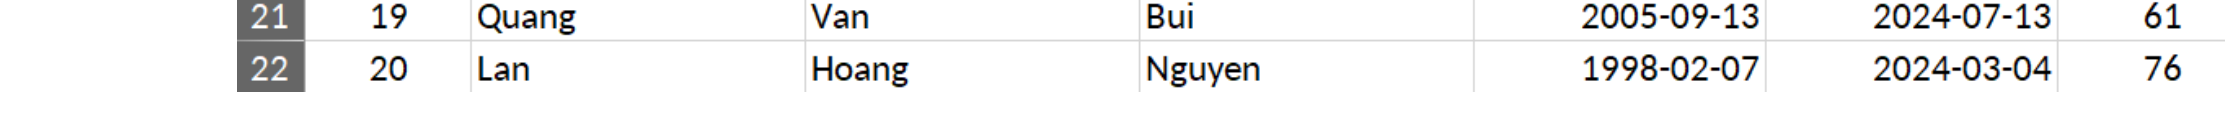
\includegraphics[width=0.92\textwidth]{assets/excel_table_sample.png}\\[4pt]
    \textit{\small Hình minh họa. Ví dụ dữ liệu trong tệp Excel}
\end{center}
\vspace{2pt}

\textbf{Ví dụ dữ liệu câu hỏi trong tệp queries.json:}

\begin{tcolorbox}[codebox]
[\newline
\hspace*{1.5em}\{\texttt{"}id\texttt{"}: 1, \texttt{"}file\_name\texttt{"}: \texttt{"}sample.xlsx\texttt{"},\newline
\hspace*{2.5em}\texttt{"}query\texttt{"}: \texttt{"}How many people have a score higher than 80?\texttt{"}\},\newline
\hspace*{1.5em}\{\texttt{"}id\texttt{"}: 2, \texttt{"}file\_name\texttt{"}: \texttt{"}sample.xlsx\texttt{"},\newline
\hspace*{2.5em}\texttt{"}query\texttt{"}: \texttt{"}What is the last name of the person with the highest score?\texttt{"}\}\newline
]
\end{tcolorbox}

\newpage

\textbf{Ví dụ kết quả tương ứng trong tệp submission.csv:}

\begin{tcolorbox}[codebox]
id,answer\newline
1,11\newline
2,Ngo
\end{tcolorbox}

Bài dự thi được đánh giá trên tập kiểm thử ẩn do BTC xây dựng theo quy trình tương tự bộ dữ liệu công khai.

Bộ dữ liệu công khai đợt 1: \textbf{\href{https://drive.google.com/drive/folders/1IiEl_weVjIdd1xlnhtiuY-NzmiThXa4o?usp=sharing}{\underline{Truy cập tại đây}}}

\textbf{3. Yêu cầu đối với bài dự thi}

\begin{itemize}[leftmargin=1.5em, itemsep=2pt, topsep=1pt, parsep=0pt, label=--]
    \item Giải pháp nhận đầu vào là thư mục chứa các tệp .xlsx và tệp queries.json; kết quả phải được xuất ra tệp submission.csv đúng định dạng mẫu.
    \item Mỗi id trong queries.json tương ứng với đúng một dòng kết quả. Trường answer chỉ ghi đáp án cuối cùng, không kèm giải thích.
    \item Mỗi đội nộp một tệp .zip gồm mã nguồn, các tệp cấu hình/phụ thuộc cần thiết và tệp README.md hướng dẫn cài đặt, cấu hình, chạy chương trình bằng dòng lệnh.
    \item Giải pháp phải có khả năng chạy lại với dữ liệu đầu vào mới, không phụ thuộc vào đường dẫn của bộ dữ liệu mẫu. Bài không chạy được hoặc không tạo ra tệp kết quả hợp lệ sẽ không được chấm.
\end{itemize}

\textbf{4. Giới hạn tài nguyên và điều kiện thực thi}

\textbf{Mô hình ngôn ngữ (LLM):} Nếu sử dụng LLM để trả lời câu hỏi, giải pháp phải hỗ trợ mô hình thống nhất khi chấm thi là Qwen3.7 Flash (model ID: qwen/qwen3.7-flash), truy cập qua OpenRouter (\href{https://openrouter.ai/qwen/qwen3.7-flash}{https://openrouter.ai/qwen/qwen3.7-flash}). Đội thi phải cho phép cấu hình thông tin truy cập API và không đưa khóa API vào mã nguồn. Quy định này không hạn chế việc sử dụng công cụ AI trong quá trình phát triển giải pháp.

\textbf{Chi phí LLM:} Tổng chi phí gọi LLM trên tập kiểm thử ẩn không vượt quá 0.10 USD/câu hỏi cho mỗi lần chấm, tính cả các lượt gọi lại (retry). Chi phí được xác định theo mức sử dụng API do BTC ghi nhận.

\textbf{Thời gian thực thi:} Tối đa 40 phút cho 20 câu hỏi, tính từ lúc bắt đầu chạy giải pháp đến khi tạo xong tệp submission.csv, bao gồm thời gian xử lý dữ liệu và gọi API. Việc chấm thi được thực hiện trên máy của BTC có cấu hình 6 core vCPU, 12 GB RAM.

\textbf{Dung lượng và bộ nhớ:} Tệp .zip nộp bài không được vượt quá 100 MB. Trong quá trình chạy trên tập kiểm thử ẩn, tổng không gian bộ nhớ giải pháp sử dụng không được vượt quá 1 GB.

\textbf{Lưu ý:} Bài dự thi vi phạm một trong các giới hạn nêu trên sẽ không được chấm điểm.

\textbf{5. Chấm điểm và xếp hạng}

BTC chạy các bài dự thi hợp lệ trên tập kiểm thử ẩn. Thứ tự xếp hạng được xác định

\newpage

theo các tiêu chí ưu tiên sau:

\begin{enumerate}[leftmargin=1.5em, itemsep=3pt, topsep=2pt, label=\textbf{\arabic*)}]
    \item \textbf{Số câu trả lời đúng theo so khớp chính xác với đáp án chuẩn (Exact Match):} đội có nhiều câu trả lời đúng hơn được xếp trước.
    \item \textbf{Thời gian thực thi trung bình mỗi câu hỏi:} đội có thời gian thấp hơn được xếp trước nếu số câu trả lời đúng bằng nhau.
    \item \textbf{Số token LLM sử dụng trung bình mỗi câu hỏi:} đội dùng ít token hơn được xếp trước nếu hai tiêu chí trên bằng nhau.
\end{enumerate}

\textbf{6. Lịch trình}

\vspace{2pt}
\noindent
{\arrayrulecolor{tableborder}
\begin{tabularx}{\textwidth}{p{4.0cm} X}
\rowcolor{headergray}
\textbf{Thời điểm} & \textbf{Hoạt động} \\
\hline
19h00 ngày 13/10 & BTC công bố bộ dữ liệu công khai lần 1; các đội bắt đầu phát triển giải pháp. \\
\hline
09h00 ngày 16/10 & BTC công bố bộ dữ liệu công khai lần 2. \\
\hline
12h00 ngày 17/10 & Hạn cuối nộp tệp .zip chứa bài dự thi. \\
\hline
12h00--17h00 ngày 17/10 & BTC chấm các bài dự thi hợp lệ trên tập kiểm thử ẩn. \\
\hline
20h00 ngày 17/10 & Công bố bảng xếp hạng tạm thời. \\
\hline
08h00-17h00 ngày 18/10 & Vấn đáp xác minh giải pháp của các đội thi. \\
\hline
20h00 ngày 20/10 & Công bố bảng xếp hạng chính thức. \\
\hline
\end{tabularx}
}
\vspace{8pt}

\textbf{7. Vấn đáp và xác minh}

Phần vấn đáp nhằm xác minh mức độ làm chủ giải pháp của đội thi. Các đội phải giải thích được nguyên lý hoạt động, các thành phần chính và chứng minh khả năng điều chỉnh mã nguồn theo yêu cầu phù hợp với phạm vi đề thi. Đội không đáp ứng yêu cầu xác minh sẽ bị loại khỏi bảng xếp hạng chính thức.

\end{document}
